% !TEX root = ../paper.tex

%\section{Background}
%In this section, we describe MCR process based on Gerrit system. Then, we describe the background behind our approach composed of text mining techniques using VSM and euclidian distance and prediction evaluation techniques. 
%\dan{this section seems to only cover MCR. We could have this be a Background section with this and the other subsequent sections moved to sub-sections}

\section{Modern Code Review Process}

An overview of MCR process based on the Gerrit code review system is shown in Fig. \ref{fig:process}.
The grey area shows the review process of the system which is composed of four main steps:
(1) An author creates a patch and submits a set of new or modified files as a review request to the Gerrit system.
(2) Reviewers examine the proposed code changes for defects or concerns.
(3) Reviewers provide comments to the author.
The author creates a revised proposed change according to the comments and re-submits for review.
Reviewers then examine the revised proposed change.
If the revision is not approved, reviewers provide comments to fix and the process continues until
(4) reviewers can determine that a proposed change can be merged into the project (approved change) or should not be merged (rejected).


According to this process, reviewers' comments are the most important factor in determining software quality.
In particular, McIntosh et. al. \cite{Mcintosh} found that components which were reviewed without discussion (i.e. no comments) are likely to contain bugs.
However, it has not been shown that components with comments are less likely to contain bugs. Tools supporting MCR such as Gerrit allow reviewers to freely write messages to authors (and other reviewers), and frequently, these comments are superficial or do not clearly identify defects or relevant issues for the proposed change and are thus of questionable usefulness and consequently may have little impact on quality.
% (e.g. coding styles, documentation, process workflow, etc.)
For example, a comment may be related to something outside the scope of the proposed change, perhaps author or reviewer personal issues or inter-personal communication e.g. ``Keep up the good work everyone!".
Microsoft developers reported that the reviewers often only focus on minor logic errors rather than discussing deeper design issues \cite{Bacchelli2013a}.
Our observations of the Qt project also corroborate this finding.
We found that many examples of comments that are superficial and unhelpful to the proposed changes.
For example, the superficial and unconfident comment shown in Fig. \ref{fig:example}(a) is certainly within the scope of the proposed change, yet provides little useful information.
While the comment in Fig. \ref{fig:example}(b) about using the version control system (in this case Git) is clearly out of scope, and not directly useful for the proposed change. 

Ultimately, our aim is to understand the impact of useful and useless comments on code quality. Specifically, what degree of useful comments are needed to effect positive impact on quality. Study of this necessitates ascertaining, with high confidence, the usefulness of a large number of comments. This  had proven difficult to accomplish manually, so here we investigate the pragmatics of using semantic similarity to assist with this task.


\begin{figure}[!t]
\centering
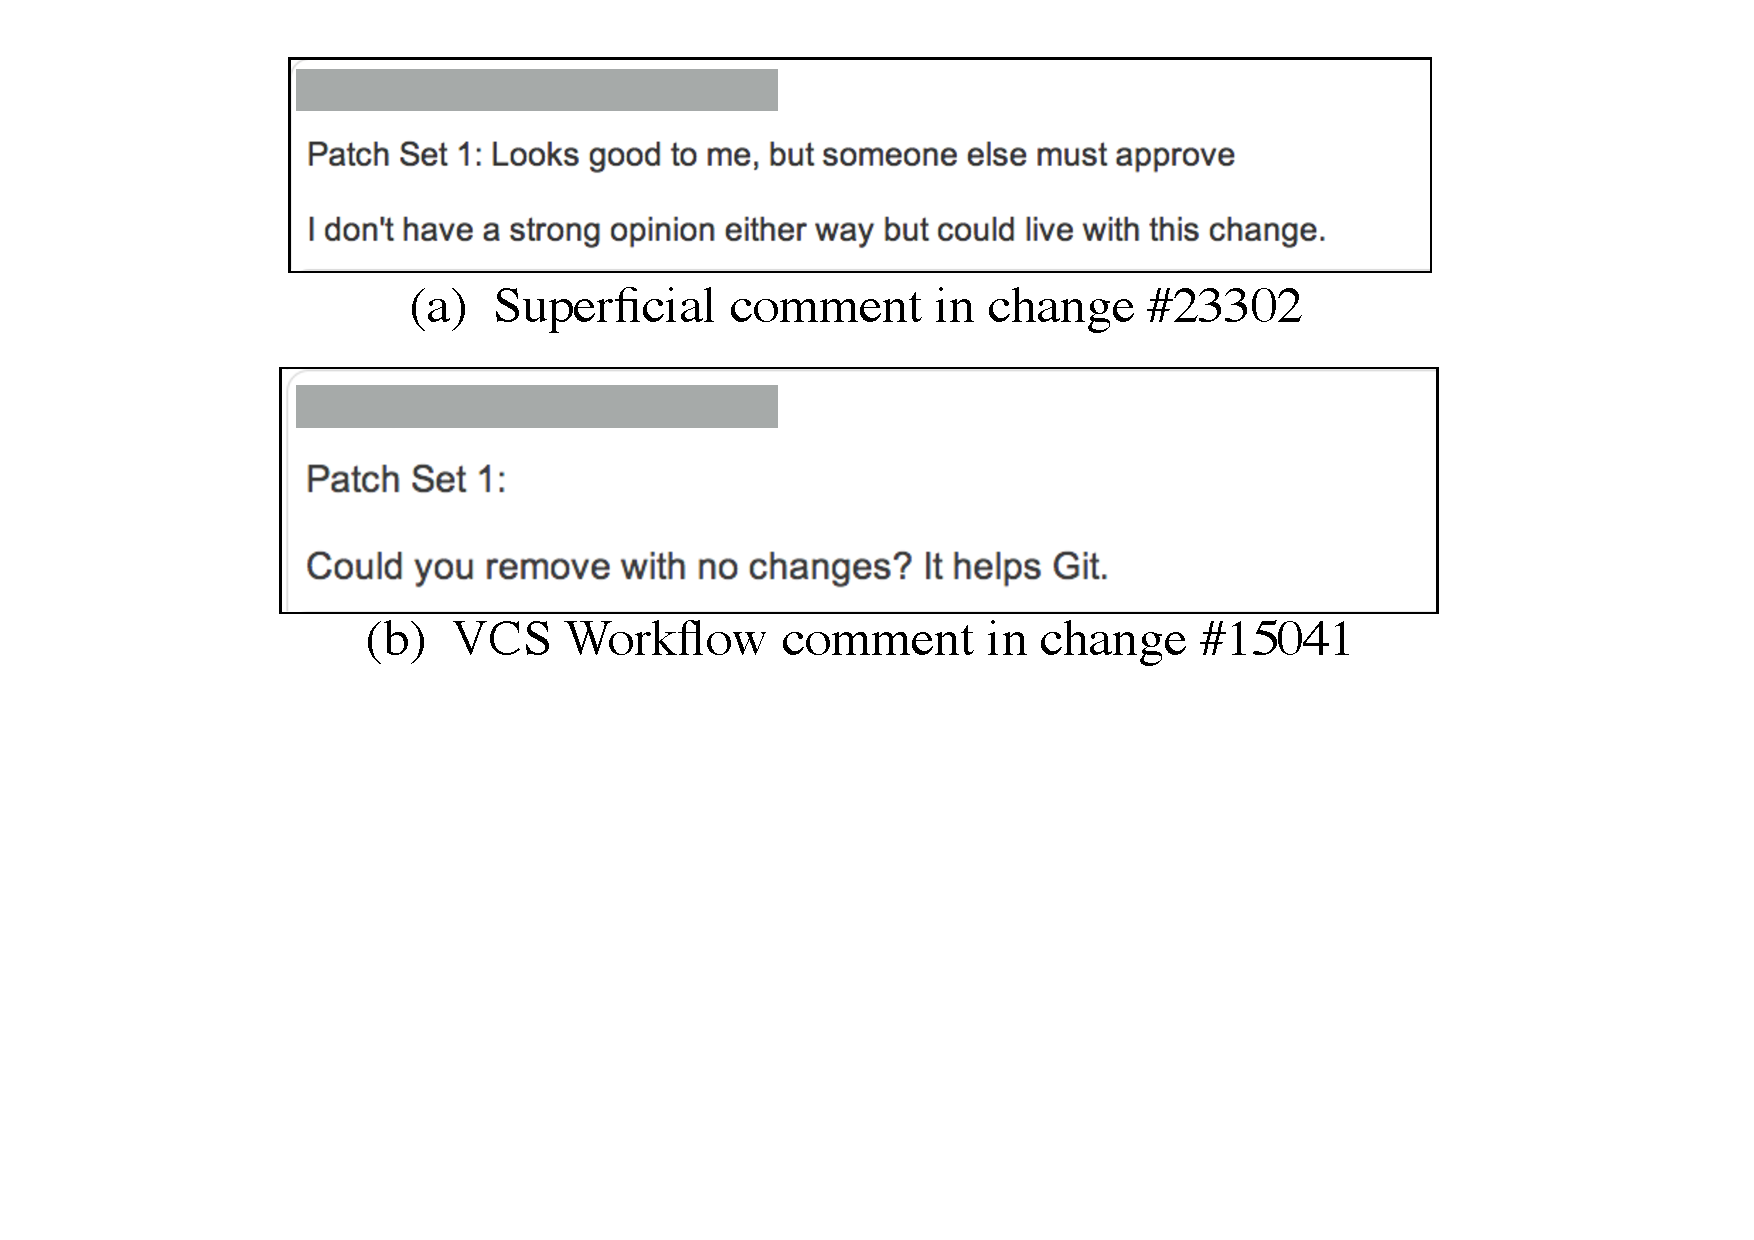
\includegraphics[scale=0.33, trim= 100 250 0 0, clip=true]{comment_examples}
\caption{Examples of comment in code reviews of Qt project.}
\label{fig:example}
\end{figure}
